
\chapter{Dimensional Reduction and Visualization Improvements}

Purpose:



\section{Dimensional Reduction}

\subsection{Principal Component Analysis}

Tharrault paper

Russell paper

\section{Meta-Analysis}

\subsection{Out-of-Family Telemetry}

Two NASA papers

\subsection{Out-of-Family Correlations}



\section{Corrgram Enhancements and Dimensional Reduction}

\subsection{Smoothing and Time Adjustments}

\subsection{Ranked Filtering}

\subsection{Fault Filtering}

\subsection{Substring Filtering}

\subsection{Cross-System Filtering}

\subsection{Timelines}


\section{Two-Dimensional Graph Embeddings}

Since the vast majority of user interfaces in common usage are two-dimensional, and hardware limitations can easily result in 3D user interfaces being infeasible for users, it makes sense to look at ways that $n$-dimensional system state data can be embedded within a 2D visualization. Towards this purpose, I did a brief survey of state-of-the-art 2D graph embeddings, looking for implementation feasibility and the ability to give a user ``insight" into the nature of a system fault. Preferably, a 2D embedding for system understanding will make major state transitions and patterns visibly obvious at a glance, and will spatially separate different system ``modes" so that they can easily be mentally grouped by the viewer.

\subsection{Undirected Dependency Graphs}

The first type of two-dimensional graph embedding that we examined as an alternative for animated corrgrams was the ``dependency graph." Dependency graphs are a type of 2D embedding in which a complex system is represented as a directed graph, where nodes are system components and edges represent dependencies; for example, if $\textbf{node}_{A} \rightarrow \textbf{node}_{B}$ and $\textbf{node}_{B} \rightarrow \textbf{node}_{C}$, this indicates that the value of $\textbf{node}_{A}$ depends on the value of $\textbf{node}_{B}$, which in turn depends on $\textbf{node}_{C}$. A simple example of this type of visualization is shown in Fig.~\ref{fig:dependency_graph_example}.

\begin{figure}[h]
\centering
    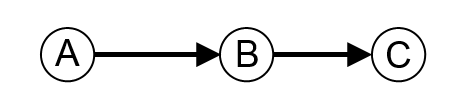
\includegraphics{images/dependency_graph_example.png}
    \caption{A simple example of a traditional dependency graph is shown. Here, node A's value depends on the value of node B, and node B's value depends on the value of node C.}
    \label{fig:dependency_graph_example}
\end{figure}

As such, this type of visualization lends itself well to illustrating the effect of causation in a system. Though causation can be difficult to determine in a complex system, as we have already shown, correlation is calculable via the PCC and other metrics, and a correlation-generalized undirected correlation graph could be envisioned, wherein two nodes have an undirected edge if their mutual PCC score exceeds a certain threshold, and have no edge if their mutual PCC score fails to meet that threshold. The steps to generate such a graph are as follows:

\begin{enumerate}
    \item At a given point in time, generate a PCC matrix for all of the possible data channel pairs.
    \item Generate an unconnected graph in which there exists a degree-0 node for each data channel.
    \item For node-node pair, add a connecting edge if there exists a PCC score above a reasonably high correlation threshold (e.g., $r_{PCC}^{2} > 0.8$). This edge can be colored to show correlation sign (e.g., blue for $r_{PCC} < 0$ and red for $r_{PCC} > 0$).
    \item Finally, cull all nodes that are still of degree 0.
\end{enumerate}

With the corrgram visualization, we needed to illustrate all possible pairs of channels as a separate cell, and thus ended up needing to visualize $\frac{n!}{2 (n - 2)!}$ different cells (where $n$ is the number of data channels). However, with a dependency graph visualization, we can reduce the number of colored elements (nodes) to a count of $n$, by introducing connecting edges. (For systems that are not highly correlated, this will produce far less visual clutter than the corrgram visualization.) Furthermore, we can simplify the undirected dependency graph visualization by eliminating any components of degree 0, if the correlated components are the only ones we wish to see.

We experimented with actually creating this visualization for explorational purposes. First, we ran a system dynamics simulation for our lunar rover described in Chapter 5. We paused the telemetry analysis at a certain time step at which interesting correlated components were present, and examined the data channel correlations at that instant. The correlated components are illustrated in the correlation map visualization in Fig.~\ref{fig:comparison_correlation_map}. We then isolated the correlated components and illustrated them as an undirected dependency graph, using the steps outlined above. The resulting undirected dependency graph visualization, with positive and negative correlation edges both visible, is shown in Fig.~\ref{fig:undirected_both}. In addition, positive and negative correlated components have been isolated into separate graphs for readability and discoverability, as shown in Fig.~\ref{fig:undirected_positive_only} and Fig.~\ref{fig:undirected_negative_only}, respectively.

\begin{figure}[h]
\centering
    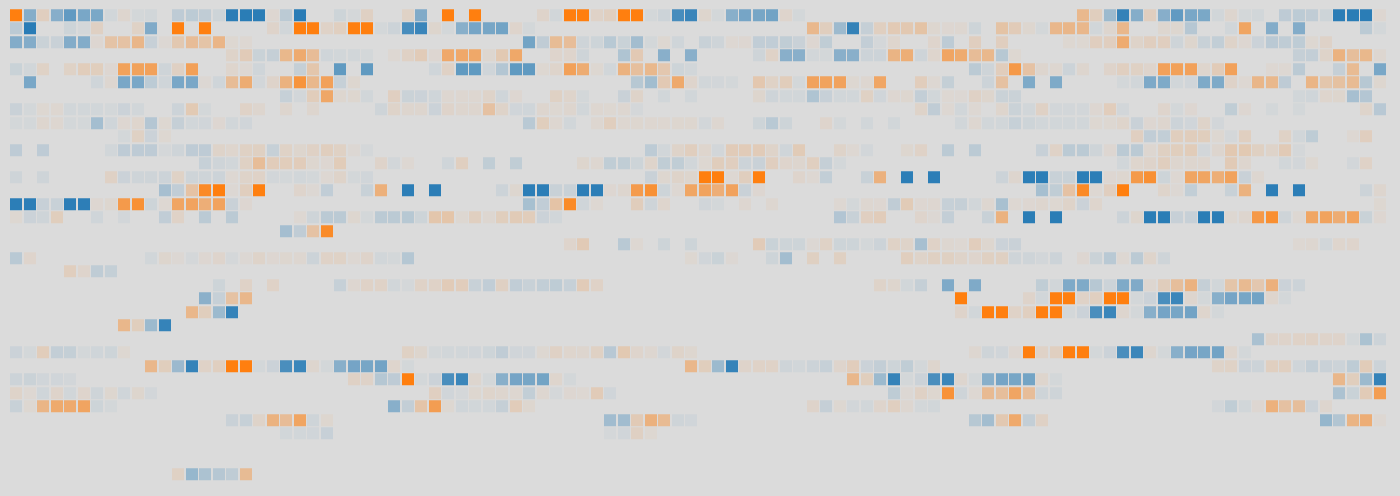
\includegraphics[width=\columnwidth]{images/comparison_correlation_map.png}
    \caption{A snapshot of the correlation map display from a simulated run. Note the strong correlations illustrated by opaque orange (positive) and blue (negative) cells.}
    \label{fig:comparison_correlation_map}
\end{figure}

\begin{figure}[h]
\centering
    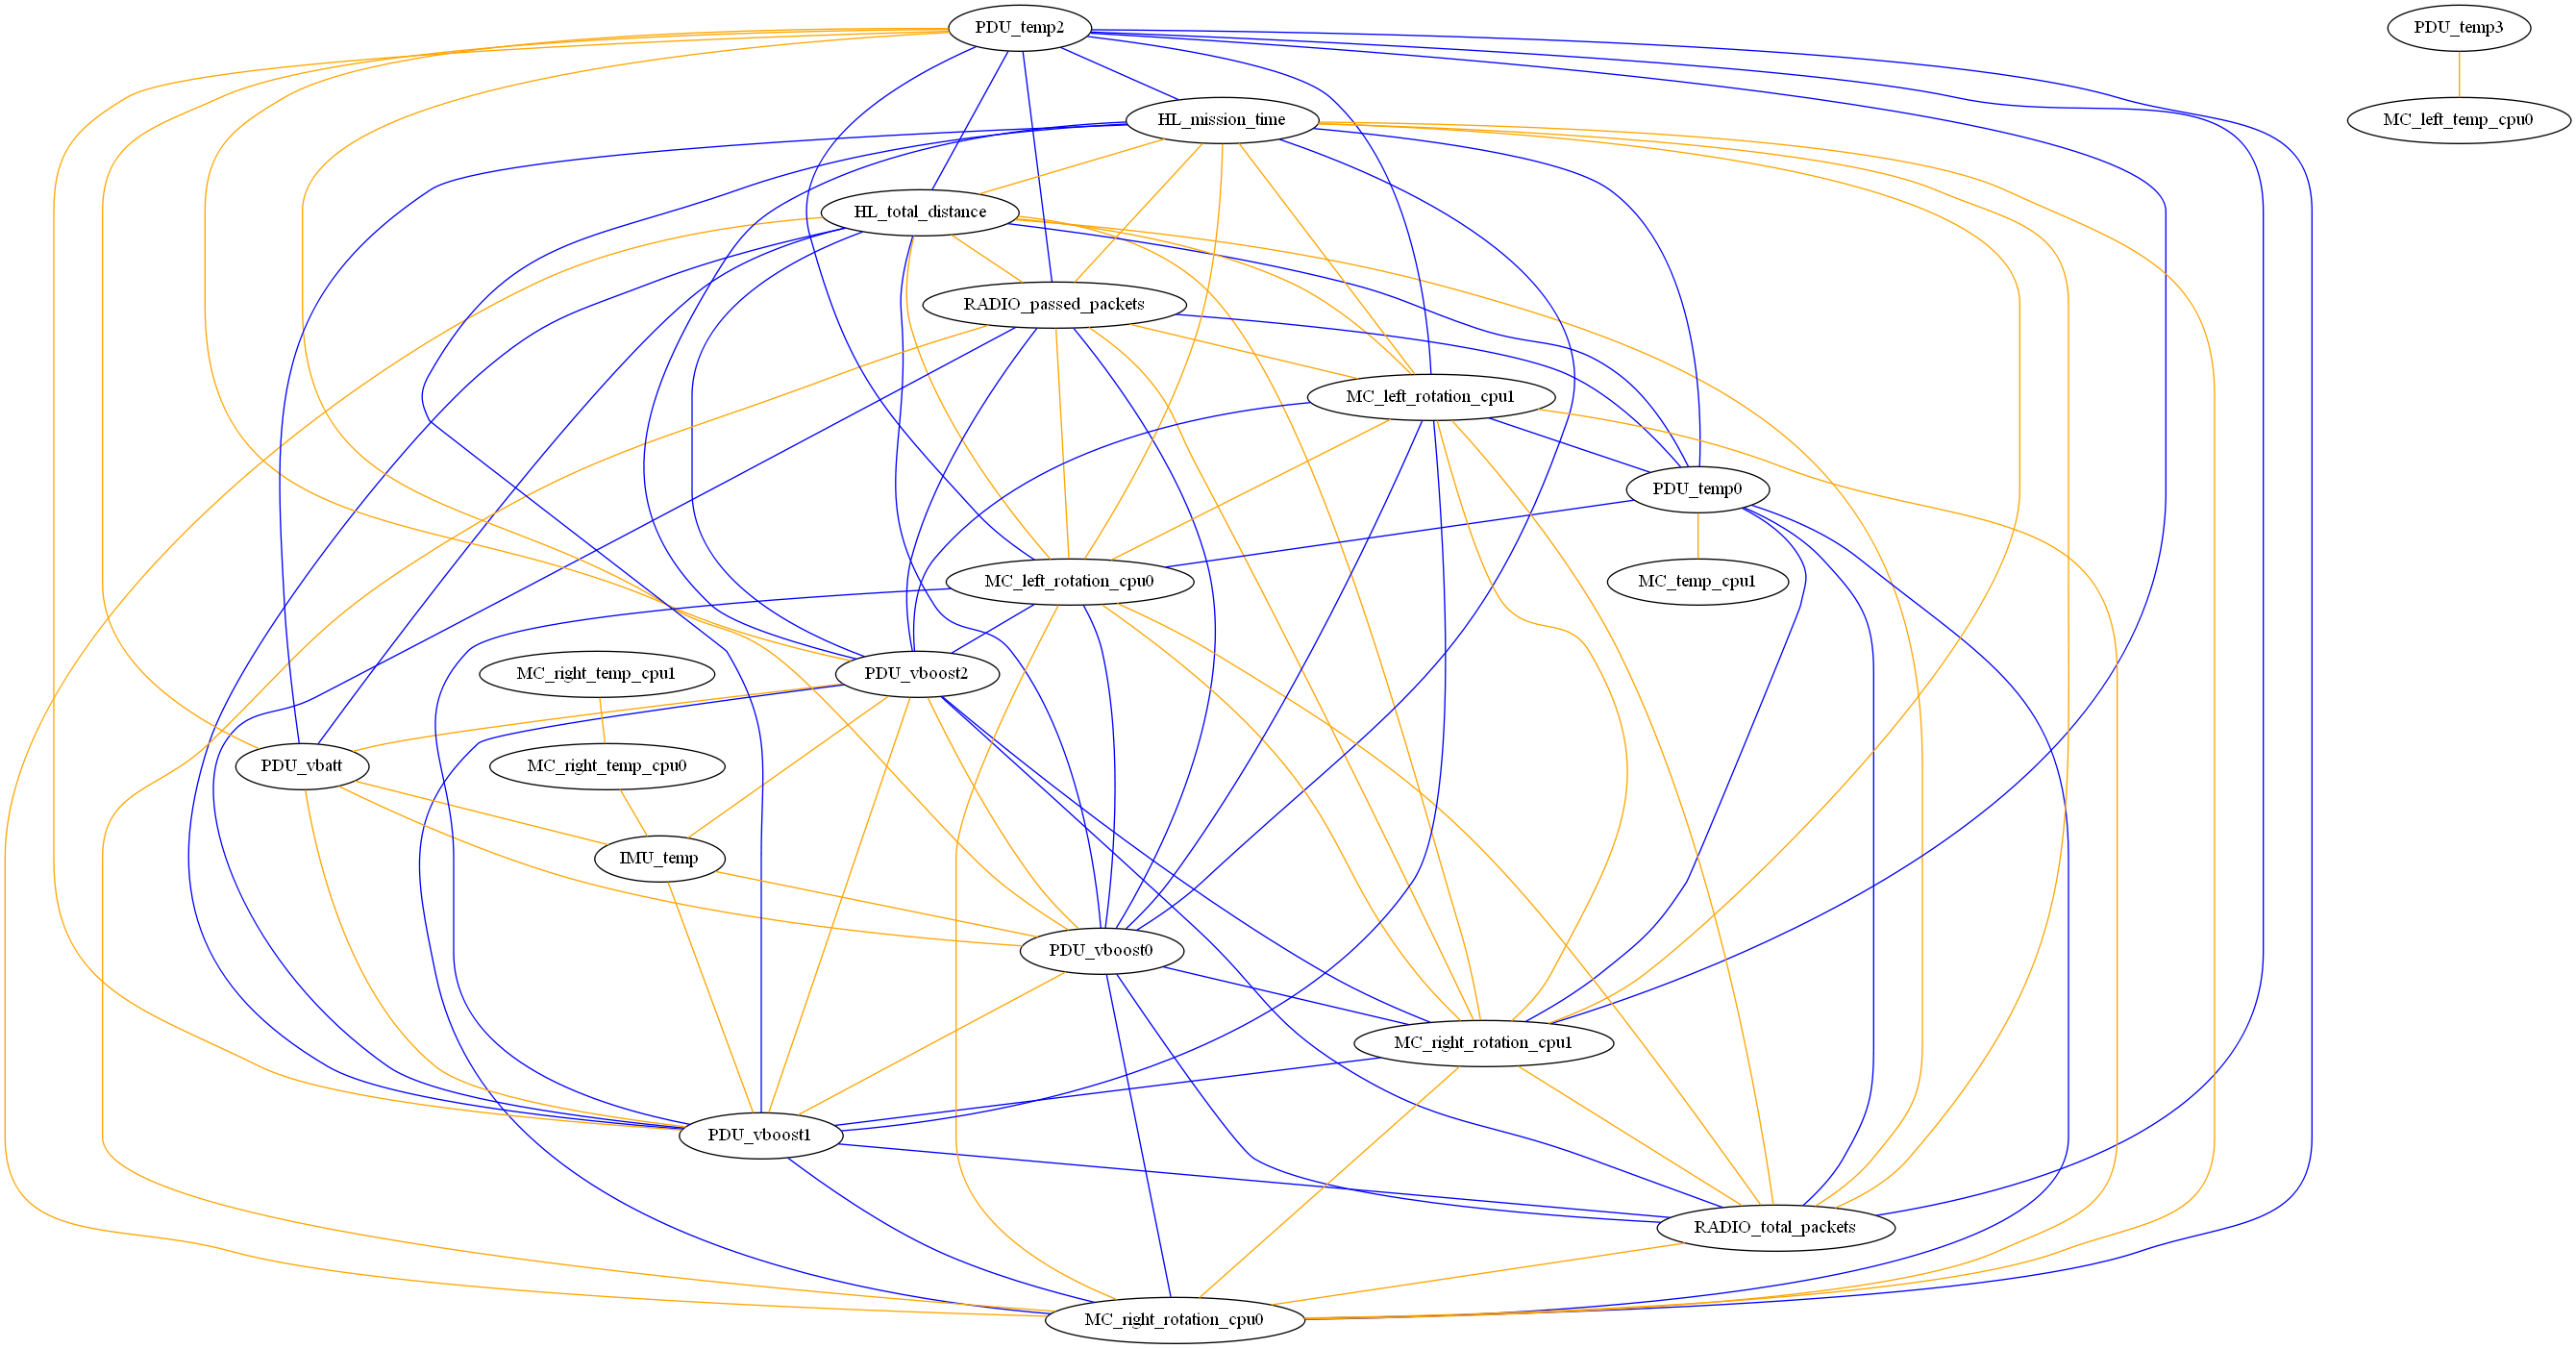
\includegraphics[width=\columnwidth]{images/undirected_both.png}
    \caption{A snapshot of an undirected dependency graph display from a simulated run. Correlated components have been isolated, with edges drawn for all correlation relationships exceeding a certain value ($r_{PCC}^{2} > 0.8$). Both positive and negative correlation connections are shown. Self-correlations are not shown.}
    \label{fig:undirected_both}
\end{figure}

\begin{figure}[h]
\centering
    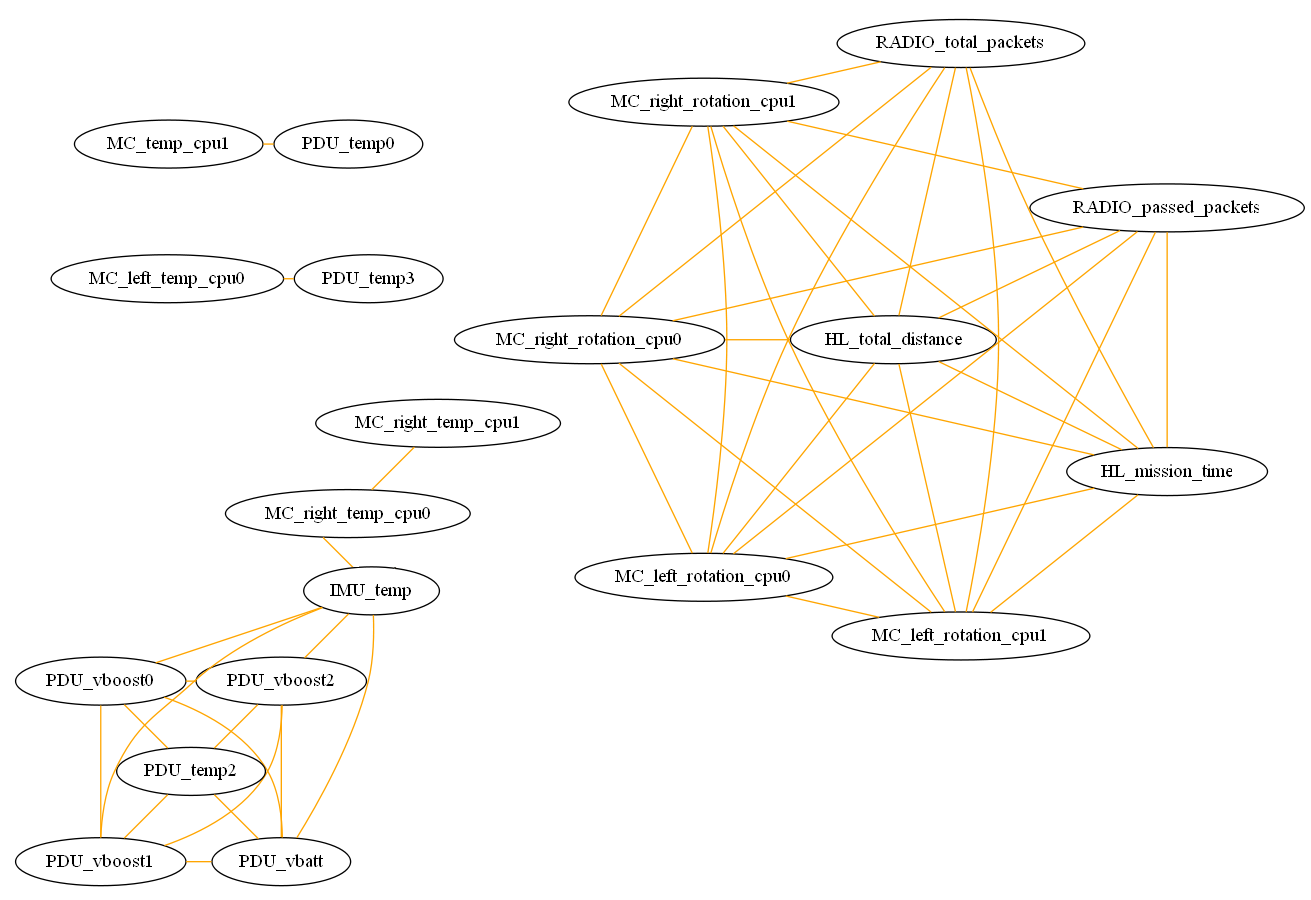
\includegraphics[width=\columnwidth]{images/undirected_positive_only.png}
    \caption{A snapshot of an undirected dependency graph display from a simulated run. Correlated components have been isolated, with edges drawn for all correlation relationships exceeding a certain value ($r_{PCC}^{2} > 0.8$). Only positive correlations are shown. Self-correlations are not shown.}
    \label{fig:undirected_positive_only}
\end{figure}

\begin{figure}[h]
\centering
    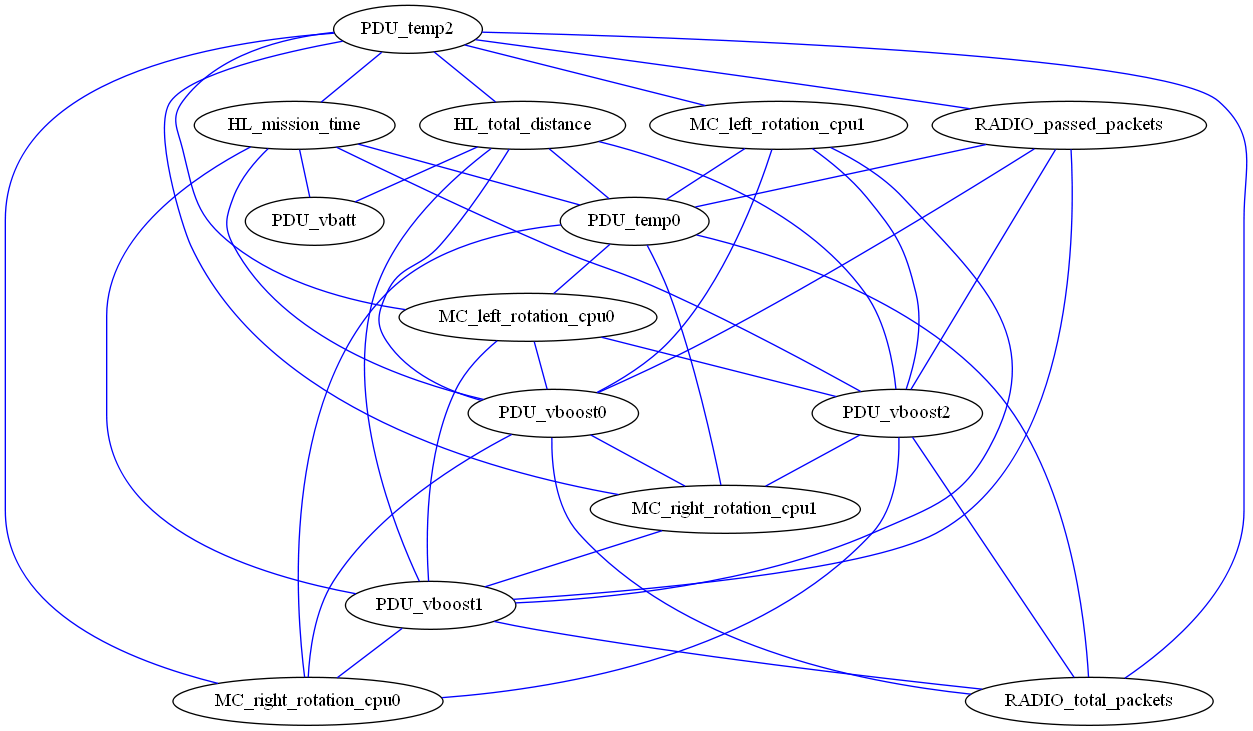
\includegraphics[width=\columnwidth]{images/undirected_negative_only.png}
    \caption{A snapshot of an undirected dependency graph display from a simulated run. Correlated components have been isolated, with edges drawn for all correlation relationships exceeding a certain value ($r_{PCC}^{2} > 0.8$). Only negative correlations are shown. Self-correlations are not shown.}
    \label{fig:undirected_negative_only}
\end{figure}

These visualizations present a very different way of viewing the correlative data. While the temporal dimension is still only captured as a snapshot (i.e., the correlative state at only one time point can be shown at a time), correlated components are shown very clearly, and can be understood at a glance. In particular, the intuition behind the positive correlated components in Fig.~\ref{fig:undirected_positive_only} seems clear; the most fully-connected, major clusters are exhibiting behavior which is very similar to each other. (In fact, the lower left cluster channels were all in a state of monotonic decrease, and the upper right cluster channels were in a state of monotonic increase.) The negative correlated components are less obvious, as they don't ``cluster" in the same way; however, the negative correlation data can be overlaid onto the positive correlation graphs as a higher-level operation on the clusters. This, perhaps, produces the most informative type of graph; this application is shown in Fig.~\ref{fig:undirected_positive_with_negative_clusters}.

Note that \cite{yeh2007exploratory} uses a similar approach for graph visualization of correlation matrices relationships; however, they impose a radial structure on all graph layouts, which losing the clustering advantage of the graph layouts we have produced here.

\begin{figure}[h]
\centering
    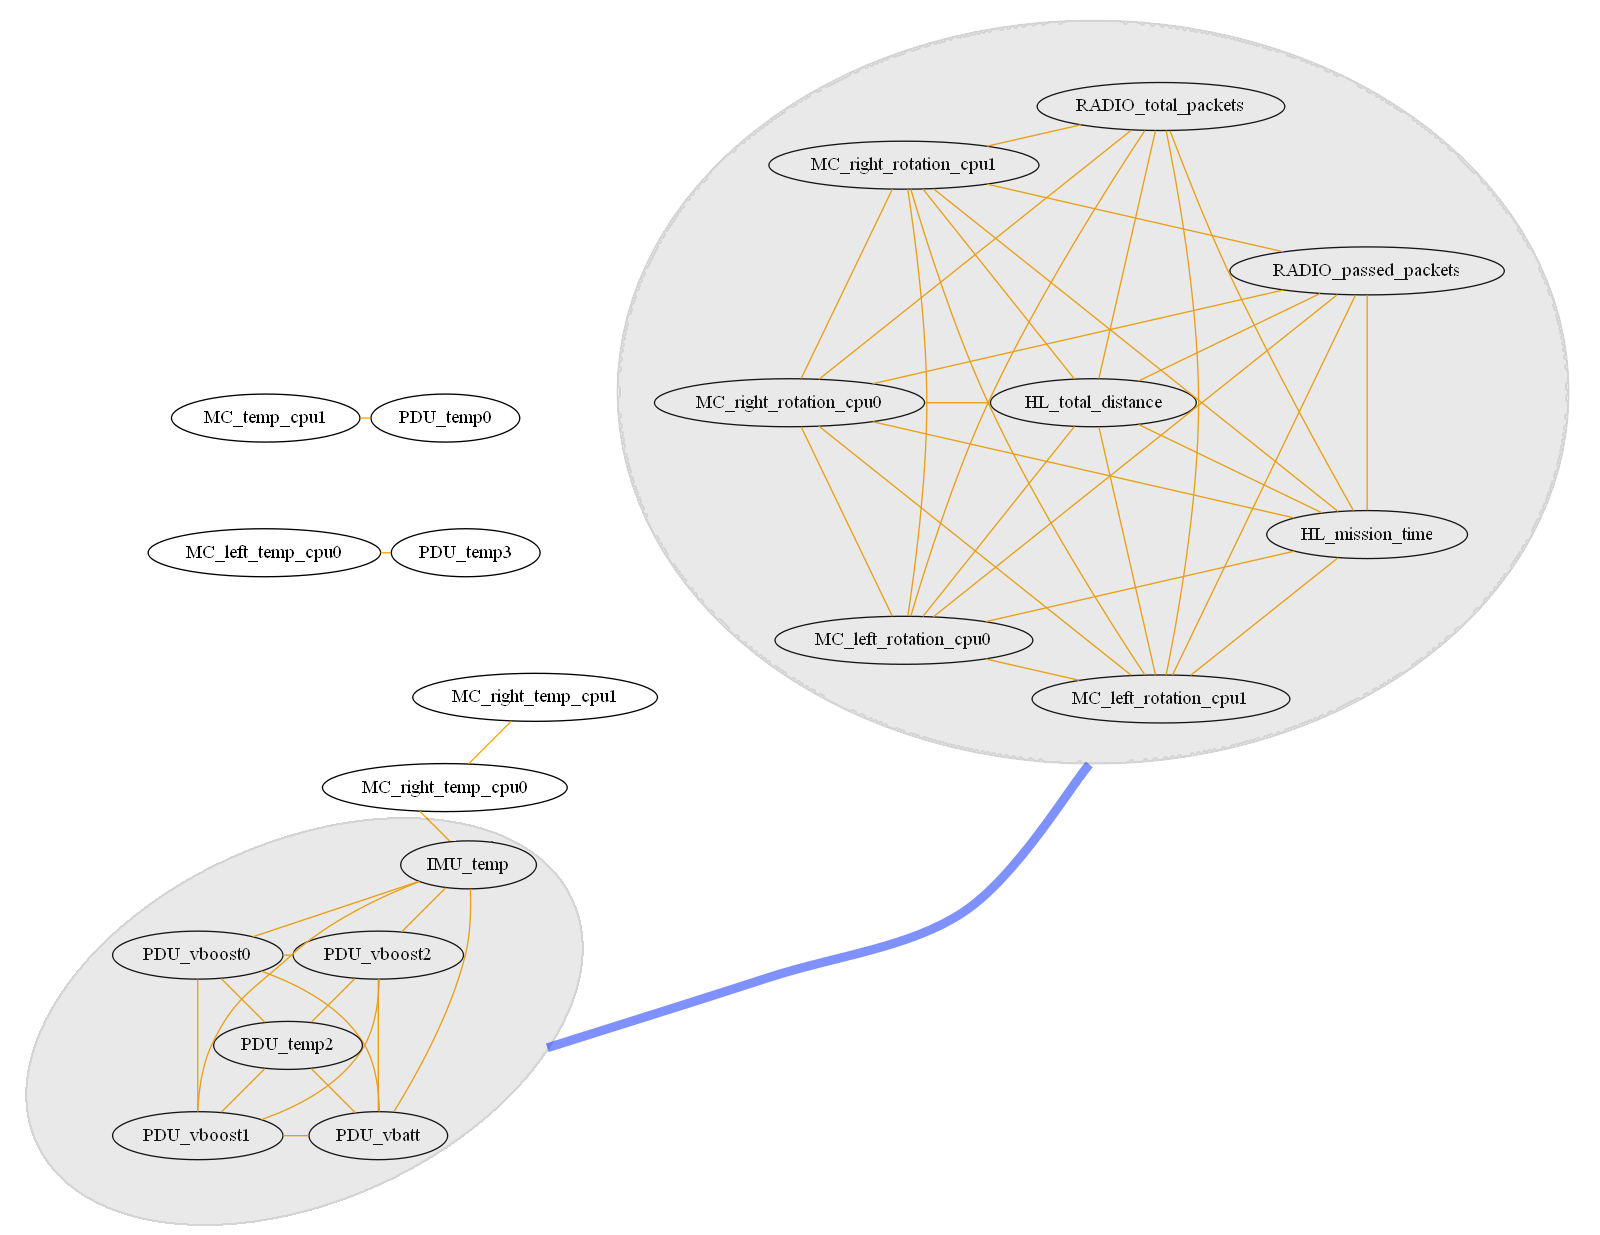
\includegraphics[width=\columnwidth]{images/undirected_positive_with_negative_clusters.png}
    \caption{A snapshot of an undirected dependency graph display from a simulated run. Correlated components have been isolated, with edges drawn for all correlation relationships exceeding a certain value ($r_{PCC}^{2} > 0.8$). Positive correlations, and negatively correlated subgraphs, are shown. Self-correlations are not shown.}
    \label{fig:undirected_positive_with_negative_clusters}
\end{figure}

Another advantage of this technique is that it clearly isolates small groups of correlated components; low-degree subgraphs can point towards noisy data, or towards significant links, but if they are persistent, it seems they may suggest interesting correlations that deviate from the patterns exhibiting by the bulk of the data channels, which tend to correlate due to behavior exhibiting positive and negative monotonicity. However, towards the idea of exploring a visualization which can show the evolution of state and correlative data over time, we will look at another technique in the following section.

\section{Time Curves}

In early 2016, Bach et al presented a powerful new type of visualization tool called ``Time Curves" \cite{bach2016time}. The time curve is a generic 2D embedding algorithm designed specifically for system state data which changes over time. Time curves visualize system states as a series of points, connected in temporal along curves within the 2D embedding. This allows the viewer to gain an understanding of system behavior by the shape and directions of the curves, and by the grouping of the data points. A visual example of how a time curve is ``folded" from an initial linear timeline is shown in Fig.~\ref{fig:time_curve_example}.

\begin{figure}[h]
\centering
    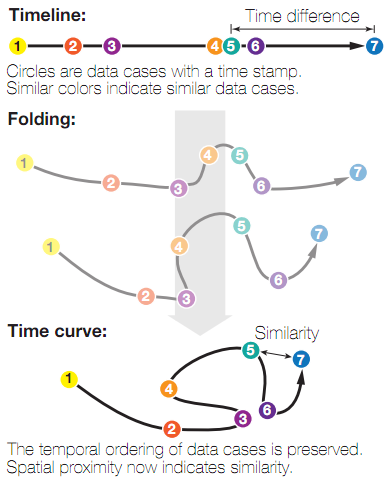
\includegraphics[width=0.5\columnwidth]{images/time_curve_example.png}
    \caption{A time curve is ``folded" from an initial linear timeline to bring similar data points close together in the 2D embedding. From \cite{bach2016time}.}
    \label{fig:time_curve_example}
\end{figure}

Let's take a closer look at how time curves model system behavior. In the time curves description, states over time are described as a series of ``time points," where each time point is a vector $\bar{x} \in \mathbb{R}^{n}$. For $t$ time points, the state at each time point can be horizontally packed into a matrix $M \in \mathbb{R}^{n \times t}$, which represents the full state history of the system.

The time curves algorithm uses a handful of multidimensional scaling (MDS) techniques which seek to map 2D Euclidean embedding distance to a user-supplied measure of vector distance, such that significantly ``similar" states are nearby in the embedding, while significantly ``different" states are far away in the embedding. The essential component to generating this embedding is the construction of a symmetric distance matrix $D \in \mathbb{R}^{t \times t}$, such that $D_{ij} = D_{ji}$ provides a pairwise distance score representing the difference between the states $M_{:,i}$ and $M_{:,j}$. A typical choice for this distance is a Euclidean norm, though many alternatives exist \cite{bach2016time}. The time curves algorithm performs an MDS optimization step to map the 2D embedding to the pairwise state distances described in $D$, producing the final visualization.

The time curves algorithm has many characteristics which make it an appealing candidate for complex system visualization. It exhibits \textbf{clustering}, where time points of similar states gather at very close points in the embedding. The viewer's eye naturally processes these clusters as single groups, and they may easily map to system modes. Time curves visualize \textbf{cycles}, where a time curve comes back to an earlier point in the embedding after moving elsewhere. This is very useful for modeling cyclic dynamics in complex systems. Time curves also emphasize \textbf{transitions} between clusters of points, as the embedding naturally pushes distinct clusters geometrically apart from each other.

Finally, time curves are very extensible, and can be combined with higher-level data which provides further insight into the state at a given time point.

\section{Applying Time Curves to System Telemetry Data}

We set about applying time curves to complex system telemetry data, in order to compare visualization results for raw state telemetry and correlative states, and to see if anomalous system modes could easily be identified in the resulting embeddings. Our data processing pipeline for raw state telemetry visualization was as follows:

\begin{enumerate}
    \item At regular intervals (e.g., once per second), record the telemetered system state into a vector $\bar{x} \in \mathbb{R}^{n}$.
    \item Once the mission is complete, horizontally concatenate all state vectors to produce a state history matrix $M \in \mathbb{R}^{n \times t}$.
    \item Generate a symmetric distance matrix $D \in \mathbb{R}^{t \times t}$, such that $D_{ij} = D_{ji}$ provides a pairwise distance score representing the difference between the states $M_{:,i}$ and $M_{:,j}$.
    \item Use the time curves algorithm to generate a 2D embedding of the $t$ states described in $D$.
\end{enumerate}

In contrast, our pipeline for generating visualizations for correlated telemetry was as follows:

\begin{enumerate}
    \item Generate a state history matrix $M$ as with the raw state telemetry case.
    \item For a given window size $w$, generate windowed ``sample matrices" $W \in \mathbb{R}^{n \times w}$, such that $W_{i} = M_{:, i:i+15}$.
    \item For each windowed matrix $W$, generate a correlative matrix $R \in \mathbb{R}^{n \times n}$ (via PCC, Spearman's Rho, or Kendall's Tau), such that $R_{ij}$ gives the correlation score of $W_{i,:}$ and $W_{j,:}$. (Note that incalculable correlations, such as those with data channels of zero variance, are set to be 0.)
    \item Flatten each windowed matrix $R$, and concatenate them horizontally into a matrix $C \in \mathbb{R}^{n^{2} \times (t - w)}$, such that each column of $C$ represents the total correlative state of the system at a time point.
    \item Generate a symmetric distance matrix $D \in \mathbb{R}^{(t - w) \times (t - w)}$, such that $D_{ij} = D_{ji}$ provides a pairwise distance score representing the difference between the states $C_{:,i}$ and $C_{:,j}$.
    \item Use the time curves algorithm to generate a 2D embedding of the $(t - w)$ states described in $D$.
\end{enumerate}

The algorithms described above were applied on the user testing data set used previously during user evaluations. This data set closely simulates telemetry from a lunar mission, in which the events described in Tbl.~\ref{tbl:events} take place at pre-set times. Each of these events triggers numerous differences in simulated environment state, which in turn causes major sensor data differences. High levels of Gaussian white noise have been introduced into the sensor data to approximate real sensor behavior.

The annotated time curve visualization of the raw state telemetry progression is shown in Fig.~\ref{fig:pfm2_raw_data_time_curve_annotated}. Similarly annotated visualizations of the PCC, Spearman's Rho, and Kendall's Tau correlative state are shown in Figs.~\ref{fig:pfm2_pcc_time_curve_annotated}, \ref{fig:pfm2_rho_time_curve_annotated}, and \ref{fig:pfm2_tau_time_curve_annotated}, respectively. (These correlative visualizations were generated with a 15-second time window.)

\section{Discussion}

The time curves visualization does a pleasing job of showing the varying modes of system operation, and allows the viewer to follow state progression easily. The major moves between groups of points correspond pretty much exactly to the times during the simulation when the rover started seeing telemetry differences from different environmental conditions.

It's also evident by inspection that the state progression from correlative analysis in Figs.~\ref{fig:pfm2_pcc_time_curve_annotated}, \ref{fig:pfm2_rho_time_curve_annotated}, and \ref{fig:pfm2_tau_time_curve_annotated} is more distinct and easy to understand than that visualized using raw telemetry in Fig.~\ref{fig:pfm2_raw_data_time_curve_annotated}. We believe that there are several reasons for these core differences. First, monotonically increasing data channels (e.g., time or wheel rotations) can make it hard to isolate modes, as state vectors containing this data appear to represent different states at each time step, even when they really only indicate one mode of behavior. These data channels can ``smear" the state across a 2D embedding, due to a steady, constant distance introduced through these increasing channels. Unless they are deliberately removed from the data--which could, as a side-effect, remove valuable data crucial to understanding system behavior--these data channels will result in behavior like that seen in Fig.~\ref{fig:pfm2_pcc_time_curve_annotated}, where the initial state and final state are actually very similar system modes, but are distint within the 2D embedding.

Additionally, changing environmental dynamics, and thus, the inputs into the system, can change as the environment changes, but if the vehicle continues to handle them in the same way, then the correlative relationships among its data channels may maintain more consistency in spite of these changing dynamics. Correlative analysis, in this way, allows a human operator to more directly investigate internal system relationships (although external dynamics still manifest themselves in the correlative data as correlations of sensor value behavior with time and other monotonically increasing values).

Finally, it appears that the correlative calculations, as they act on a large time window, appear to have had a denoising side-effect on the data, and allow real changes in correlation to clearly ``push" the time points around the embedding, making state transitions more clear--while state transitions within the raw telemetry visualization are subtle and mostly buried in the rest of the data.

Another interesting observation about the data produced, in particular visible within the correlative time curve visualizations, is the presence of additional states not foreseen in the event timeline, such as the cluster of time points between events \textbf{1} and \textbf{2}. Upon close analysis, this cluster of time points appears to be a ``hallucinated event," as a side-effect of several fault states being triggered at the same time and cascading effects on telemetered measurements as temperatures and generated voltages drop. The application of the PCC correlative algorithm emphasizes this state, likely because of its limitations with respect to accurately capturing nonlinear associations and the coarse, ordinal nature of a large amount of the discrete telemetry data.

\begin{table}[]
\centering
\begin{tabular}{lll}
Event Number & Timestamp & Event Description \\
0 & 0s & Rover begins traveling forward along smooth terrain. \\
1 & 188s & Rover enters crater; begins descending into crater. \\
2 & 287s & Rover enters shade, causing temp, comms, and power drops. \\
3 & 300s & Rover begins traversing smooth bottom of crater. \\
4 & 330s & Rover begins climbing out of crater. \\
5 & 343s & Rover exits shade; continues uphill. \\
6 & 534s & Rover emerges from crater and enters smooth terrain. \\
7 & 594s & Rover enters choppy terrain. \\
8 & 643s & Rover wheel has fault; rover stops moving.
\end{tabular}
\caption{Events during a visualized user simulation are shown. Cross-reference ``Event Numbers" with labels in Figs.~\ref{fig:pfm2_pcc_time_curve_annotated}, \ref{fig:pfm2_tau_time_curve_annotated}, \ref{fig:pfm2_rho_time_curve_annotated} and \ref{fig:pfm2_raw_data_time_curve_annotated} to see correspondence.}
\label{tbl:events}
\end{table}

\begin{figure}[h]
\centering
    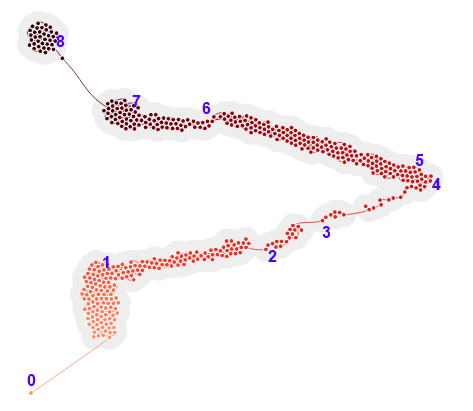
\includegraphics{images/pfm2_raw_data_time_curve_annotated.png}
    \caption{A time curve embedding visualizing mission events using raw telemetry state. Event annotations are described in Tbl.~\ref{tbl:events}.}
    \label{fig:pfm2_raw_data_time_curve_annotated}
\end{figure}

\begin{figure}[h]
\centering
    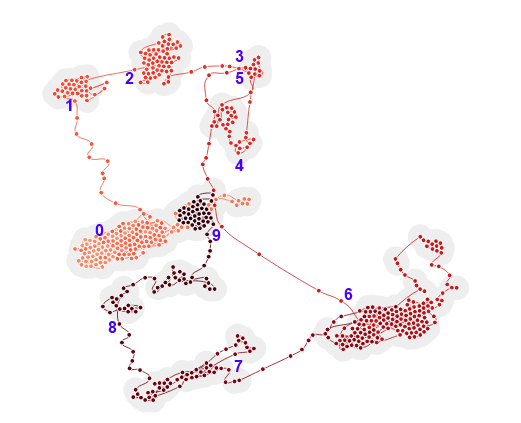
\includegraphics{images/pfm2_pcc_time_curve_annotated.png}
    \caption{A time curve embedding visualizing mission events using PCC correlation state. Event annotations are described in Tbl.~\ref{tbl:events}.}
    \label{fig:pfm2_pcc_time_curve_annotated}
\end{figure}

\begin{figure}[h]
\centering
    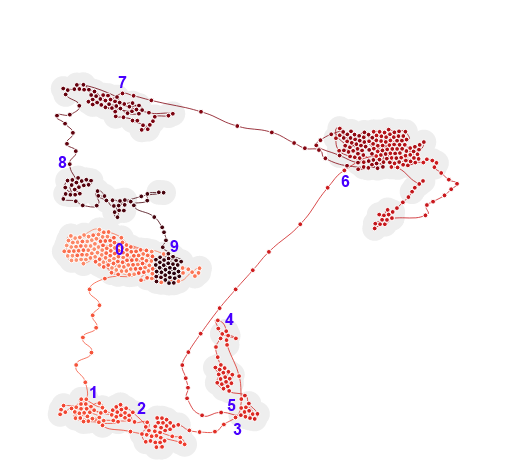
\includegraphics{images/pfm2_rho_time_curve_annotated.png}
    \caption{A time curve embedding visualizing mission events using Spearman's Rho correlation state. Event annotations are described in Tbl.~\ref{tbl:events}.}
    \label{fig:pfm2_rho_time_curve_annotated}
\end{figure}

\begin{figure}[h]
\centering
    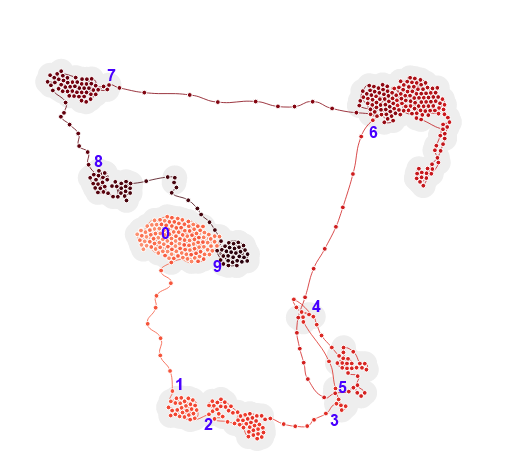
\includegraphics{images/pfm2_tau_time_curve_annotated.png}
    \caption{A time curve embedding visualizing mission events using Kendall's Tau correlation state. Event annotations are described in Tbl.~\ref{tbl:events}.}
    \label{fig:pfm2_tau_time_curve_annotated}
\end{figure}